\documentclass[12pt]{article}
\usepackage[utf8]{inputenc}
\usepackage[T5]{fontenc}
\usepackage{graphicx,a4wide,framed,amssymb,amsmath,picinpar}
\usepackage{tikz}
\usetikzlibrary{decorations,decorations.pathmorphing,shadows}


\usepackage{algorithm}
\usepackage[noend]{algorithmic}


\newcommand{\source}[1]{\begin{flushright}\emph{[#1]}\end{flushright}}

\newcommand{\MakeScribeTop}[1]{
\noindent
\begin{framed}
\noindent
 Algorithmique Avancée 2018
 \hfill
 École Centrale-Supélec
 \\[1em]
 \centerline{ \Large
#1
 }
 \\[1em]
\centerline{  \it Christoph Dürr, Nguyễn Kim Thắng}
\end{framed}
}



\begin{document}
    \MakeScribeTop{PC7 : Algorithmes d'approximations}



\section{Couverture par ensembles}

\begin{figwindow}[0,r,{\hspace*{0cm}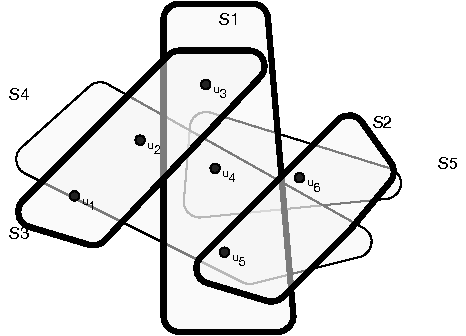
\includegraphics[width=8cm]{set_cover.pdf}},{En gras une solution possible}]
On vous donne un univers $U = \{u_{1}, \ldots, u_{n}\}$ et $m$ ensembles 
$S_{1}, \ldots, S_{m}\subseteq U$ ainsi qu'une pondération $w_{i}\in \mathbb N$ pour tout chacun des ensembles $S_i$.
Une \emph{couverture par ensembles} est une collection $\mathcal{C}$ de
ces ensembles telle que $\bigcup_{S_{i} \in \mathcal{C}} S_{i} = U$. 
L'objectif est de trouver une couverture telle que le poids total 
$\sum_{i:S_{i} \in \mathcal{C}} w_{i}$ soit minimal.	

Ce problème est NP-complet. Nous allons chercher un algorithme d'approximation.
Considérez l'algorithme suivant.
\end{figwindow}

\vspace{1cm}


\begin{algorithm}[ht]
\begin{algorithmic}[1]  
\STATE Initialement, $R \gets U$ and $\mathcal{C} \gets \emptyset$. 
\WHILE{$R \neq \emptyset$}  
	\STATE Soit $S_{i}$ un ensemble qui minimise $\frac{w_{i}}{|S_{i} \cap R|}$.
	\STATE $\mathcal{C} \gets \mathcal{C} \cup S_{i}$.
	\STATE $c_{u} \gets \frac{w_{i}}{|S_{i} \cap R|}$ pour tous $u \in S_{i} \cap R$. 
		\COMMENT{cette définition est pour l'analyse seulement.}
	\STATE $R \gets R \setminus S_{i}$.
\ENDWHILE
\STATE Retourner $\mathcal{C}$.
\end{algorithmic}
\caption{Algorithme glouton pour \textsc{Couverture des ensembles}.}
\label{algo:covering}
\end{algorithm}


\begin{enumerate}
	\item Donner une interprétation de $c_{u}$.
	\item Montrer que $\sum_{S_{i} \in \mathcal{C}} w_{i} = \sum_{u \in U} c_{u}$.
		% \item Montrer que pour chaque ensemble $S_{i}$, 
		% $
		% 	\sum_{u \in S_{i}} c_{u} \leq \left( 1 + \frac{1}{2} + \ldots + \frac{1}{|S_{i}|} \right) \cdot w_{i}
		% $
	\item Notons OPT le coût d'une solution optimale. Renommons les éléments de l'univers $U$ dans l'ordre dans lequel l'algorithme les a couverts, donc pour $i<j$, $u_i$ a été couvert en même temps ou avant $u_j$.
	Montrer que pour tout $i=1,\ldots,n$, 
		$$
			c_{u_i} \leq OPT / (n-i+1).
		$$
	\item Déduire que l'algorithme glouton ci-dessus est une $O(\log n)$-approximation.
\end{enumerate}

\section{Couverture par sommets}

\begin{figwindow}[0,r,{\hspace*{0cm}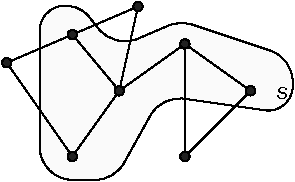
\includegraphics[width=8cm]{vertex_cover.pdf}},{Le problème de couverture par sommets.}]
On vous donne un graphe $G(V,E)$ avec $n=|V| , m=|E|$ 
et chaque sommet $v \in V$ est associé avec un poids $w_{v}$.
Une \emph{couverture par sommets} est un sous-ensemble des sommets $S\subseteq V$ tel que
chaque arête $e \in E$ a au moins une extrémité dans $S$.
L'objectif est de trouver une couverture des arêtes telle que le poids total 
$w(S) = \sum_{v \in S} w_{v}$ soit minimal.
%

Ce problème est NP-complet. Nous allons chercher un algorithme d'approximation.
Intuitivement, nous allons associer un prix $p_{e}$ à chaque arête. Les prix $p_{e}$ (pour $e \in E$) sont 
\emph{équitables} si $\sum_{e\ni v} p_{e} \leq w_{v}$ pour chaque sommet $v$; c.a.d., 
les arêtes adjacentes à $v$ ne payent pas plus que le poids du sommet $v$. 
\end{figwindow}

% \begin{enumerate}
% \end{enumerate}

 % Etant donné les prix $p_{e}$ pour $e \in E$, 
		Un sommet $v$ est dit \emph{saturé} si $\sum_{e\ni v} p_{e} = w_{v}$.
		Considérez l'algorithme suivant.
		
\begin{algorithm}[ht]
\begin{algorithmic}[1]  
\STATE Initialement, $p_{e} \gets 0$ pour toutes $e \in E$. 
\WHILE{il y a une arête $e = (u,v)$ telle que soit $u$ ou $v$ n'est pas saturé}  
	\STATE Choisir une telle arête $e$ arbitraire.
	\STATE Augmenter $p_{e}$ au maximum sans violer la propriété équitable.
\ENDWHILE
\STATE Retourner l'ensemble $S$ des sommets saturés.
\end{algorithmic}
\caption{Algorithme pour \textsc{Couverture des arêtes}.}
\label{algo:covering}
\end{algorithm}

\begin{enumerate}
	\item Montrer que pour chaque couverture des arêtes $S$, on a $\sum_{e} p_{e} \leq w(S)$.
	% \setcounter{enumi}{1}
	\item Prouver que l'ensemble $S$ et les prix $p_{e}$ retournés par l'algorithme satisfait $w(S) \leq 2 \sum_{e \in E} p_{e}$.
	\item Montrer que l'algorithme est 2-approximation.
\end{enumerate}

\end{document}